\chapter{压缩文件与压缩工具}
\label{archive-formats-and-tools}

\begin{intro}
  在\nameref{files-and-file-management}一章中,我们简要介绍了「压缩文件」:
  利用各种各样的压缩工具,我们可以将一组零散的文件和文件夹「打包」成一个体积稍小的文件,这个体积稍小的文件就是「压缩文件」。
  压缩文件有许多不同的种类,用来完成压缩流程的压缩工具也各有特色。看完这一部分,你或许可以找到这些问题的答案:
  \begin{itemize}
    \item 为什么压缩文件还有这么多种?它们的区别有哪些?
    \item RAR 格式为什么这么特殊?我电脑上的压缩工具为什么不能制作这种格式的压缩文件?
    \item 为什么在前文中我们建议只使用 ZIP 格式来与他人分享文件?
    \item 7z 是什么格式?它有哪些特点?
  \end{itemize}
\end{intro}

常见的压缩文件格式有 ZIP、RAR、7z 等多种,而市面上的的压缩工具(用来制作、解包压缩文件的软件)更是数不胜数。
了解这些常见压缩文件格式,并选择安装合适的压缩工具,有助于我们更好地管理自己的文件。

\section{「压缩」过程初探}

「压缩」可以将一个或多个文件及文件夹打包成一个文件,同时缩减体积。
我们用一个简单的例子来介绍「压缩」这个神奇的过程。假设我们有这样一句话:

\begin{verbatim}
Ask not what your country can do for you—ask what you can do for your country.
\end{verbatim}

如果存储 1 个字母(空格、破折号和句点也都看做一个字母)需要 1 个字节,那么这行 78 个字母的句子就需要 78 个字节才能完全存储。
但事实上,这个句子中有一半的内容都是冗余的——ask、not、what、your、country、can、do、for、you 这九个单词提供了组成这句话所需要的几乎所有东西。
因此,我们可以构造一个这样的「字典」:

\begin{table}[htb!]
  \centering\begin{tabular}{*{9}{c}}
    \toprule
    符号 & 1 & 2 & 3 & 4 & 5 & 6 & 7 & 8 \\
    \midrule
    单词 & ask & what & your & country & can & do & for & you \\
    \bottomrule
  \end{tabular}
  \caption{「字典」示例}
  \label{Compress_Dict}
\end{table}

那么这句话就变成了:

\begin{verbatim}
  1 not 2 3 4 5 6 7 8—1 2 8 5 6 7 3 4.
\end{verbatim}

原来的那个句子和现在我们手上的这串东西是完全等价的——即,只要有正确的字典,二者之间可以任意转换而不丢失任何数据。
换句话说,我们把原来的一个长句子,转换成了一份「字典」和一个短串;
而这份字典和这个短串,可以在我们需要的时候再变回原来的长句子。

\begin{figure}[htb!]
  \centering
  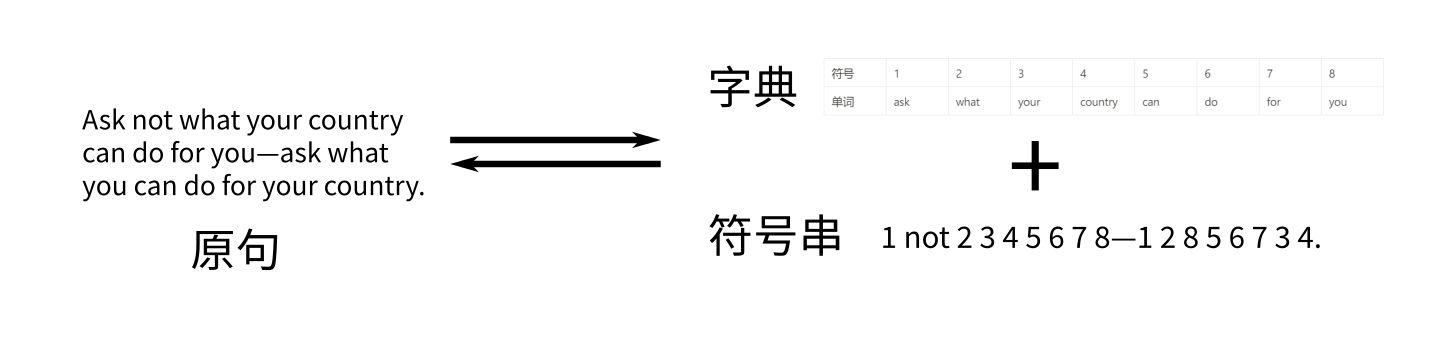
\includegraphics[width=11cm]{assets/Sentence_to_Dict.png}
  \caption{句子的「压缩」}
  \label{Sentence_to_Dict}
\end{figure}

由于字典中的「符号」是从 1 开始顺序递增的,机器可以自动地推断出来,因此存储字典需要的空间就是字典中所有单词的字母总数,为 29 个字节;
而剩下需要存储的东西就变成了极少数的几个不在字典里的单词(not、破折号和句点)以及一堆数字。
在电脑里存储这样一堆零散数字花费的空间远远少于存储之前的那些字母,因此,即使将字典的大小也一并计算,这番操作之后的「字典」加上短串的体积也小于原来的长句子。
这就是「压缩」——大体积的东西无损地变成了小体积的东西,后者可以在需要的时候变回前者。

\begin{figure}[htb!]
  \centering
  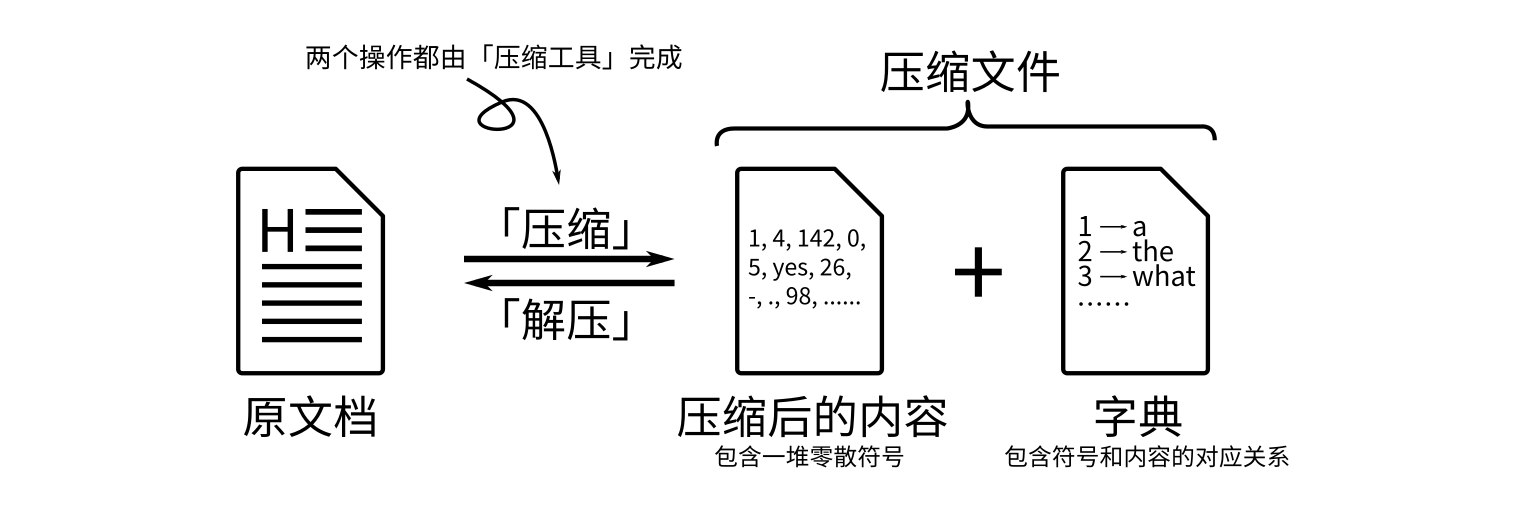
\includegraphics[width=10cm]{assets/Compressing.png}
  \caption{何为「压缩」?}
  \label{Compressing}
\end{figure}

这么看来,压缩的过程有点像数学里的「换元法」。
数学里可以用 $x$ 和 $y$ 这样的字母来替代一些复杂的、频繁出现的式子,我们只要记住 $x$ 或 $y$ 和原来式子的对应关系,就能用它们替代原先的复杂式子进行一些计算,等到合适的时候再代换回去。
这样的「对应关系」就是「字典」,代换后的式子就是「压缩文件」。

也许你会想,这个句子长得这么对称,完全是一种特殊情况,这么做是能大幅缩减空间;对于更加普遍的情况这样也适用吗?
事实上,在我们电脑上所存储的文件中——从常见的 Word 文档到各种各样的可执行文件——都包含有大量的冗余内容,这些冗余内容反复出现,完全可以用这种方式被压缩。

尽管压缩策略都是「换元法」,但具体到压缩的实现上,一千个人或许会设计出一千种方案。
首先是字典生成方法的设计。
我们需要明确,字典是压缩工具在「阅读」完整个待压缩的文件后现场编纂的。
压缩工具会以某种方式扫描所有待压缩的文件,经过一系列数学的运算后,编制出适合这些文件的高效字典。
例如,上面的例子中「not」是否编入字典,就可能影响到最终的压缩效率。
字典编得好不好,很大程度上决定了这个压缩策略的好坏。

另外,我们上面介绍的这种压缩是一种很「笨」的压缩。
举个例子,如果我们灵活地将这个句式作为一整个字典项:

\begin{verbatim}
  what ____ can do for
\end{verbatim}

其中\verb|____|是一个空位,可以放一些别的单词进去,那么可能又可以进一步省下空间——原句的前后两个分句都有这个句式。在具体的文件压缩场景中,除了「完全相同的冗余项」,「长相近似的片段」也不少,利用这种方式或许能得到更不错的压缩效率。

这就是不同压缩文件格式(或者说种类)之间产生差异的根源。
不同压缩文件格式有着不同的「压缩算法」,对应着不同的字典生成策略、「换元」策略以及更多这里没有提及的技术细节。
这些压缩文件格式有些技术公开,有的则并不公开;有的适用于一类特定文件,有的适用于另一些特定文件。
下面我们会介绍一些常用的压缩文件格式。

\section{常见的压缩文件格式}

在开始介绍这些格式之前,我们先引入一个叫做「压缩率」的概念。
假设一堆文件原来的总体积是 100 MB,在压缩成某种格式的压缩文件后,体积变成了 86 MB,就称这时的压缩率是 86\%。
压缩率不仅于压缩文件格式有关,也与源文件本身的性质有关,但我们仍然可以以「大多数工作情况下的压缩率水平」的高低来笼统地比较几种不同的压缩文件格式。

\subsection{ZIP 格式——最广泛应用的格式}

ZIP 格式可以说是「最广泛应用」的压缩文件格式——市面上任意一款压缩工具都能制作和解压这种格式的压缩文件。
即使没有安装任何压缩工具,Windows 系统也能处理这种格式的压缩包。
ZIP 格式的压缩文件扩展名是\verb|zip|。
这种格式公开于 1989 年,迄今历史悠久;又由于技术细节公开,这促成了它的广泛使用。

由于诞生的时间早,现在 ZIP 格式与其他格式相比有着许多不可忽视的缺点。
其中最明显的缺点,便是 ZIP 的压缩率不高,这是它所使用的压缩策略决定的。
然而,由于 ZIP 格式的广泛使用特性,我们仍然建议大家在与他人交换文件时,尽量使用 ZIP 格式来压缩自己的文件。

\subsection{RAR 格式——压缩率高的私有格式}

RAR 格式是一种压缩率比较高的压缩文件格式。
它的压缩文件扩展名是\verb|rar|,这种格式诞生于 1993 年。

RAR 格式的技术细节是\regcolor{不完全公开}的。
具体来说,RAR 格式的解包器是公开的,并允许以一定的方式「嵌入」在其他的压缩工具中,而\regcolor{RAR 格式的打包器则是有专利的且完全不公开}。
这意味着,市面上绝大多数的压缩工具——包括我们后文介绍的几乎所有压缩工具——都不能制作 RAR 格式的压缩包,但它们几乎都能解包这种格式的压缩包。
Windows 平台上的唯一一个能制作 RAR 压缩包的压缩工具是 WinRAR,它是收费的(可以免费试用,但有广告)。

RAR 格式的压缩率通常比 ZIP 高上不少。
除此之外,它还支持一系列其他的 ZIP 所没有的功能,例如「恢复记录」和更加安全的加密功能。
鉴于制作 RAR 格式的压缩包只能使用 WinRAR,而 WinRAR 并不是我们十分推荐的软件(有广告),因此我们不太建议大家过多使用这种格式来分享文件。

\subsection{7z 格式——高压缩率的新兴开放格式}

7z 格式是一款比较年轻(相比前面两种格式而言)的压缩文件格式。
它的压缩文件扩展名是\verb|7z|,这种格式诞生于 1999 年。

与 ZIP 一样,7z 格式的技术是完全公开的——这使得今天几乎所有的压缩软件都支持这种格式,无论是压缩还是解压缩。
不仅如此,7z 的压缩率高于 ZIP,与 RAR 几乎平分秋色,又支持高强度加密、恢复记录等附加功能,因而 7z 是一种我们十分推荐\regcolor{个人使用}(例如,将自己的文件打包存档)的格式。

然而,7z 作为后起之秀,自然没有 ZIP 或是 RAR 那样高的认可度。
至少目前,在大多数人们的学习和工作中,这种格式运用的还比较少。
故我们将 7z 推荐为「个人使用」——如果你想把一些文件打包发给别人(尤其是对方并不很懂电脑的情况下),ZIP 或许是更好的选择。

\section{压缩工具 / 压缩软件}

Windows 自身的文件管理器只能打开、解压和制作 ZIP 格式的压缩包,因此我们有必要安装额外的压缩工具软件来满足使用需求。压缩工具(压缩软件,下同)是一类特殊的软件。这种软件安装之后,你的电脑就可以查看、解压、制作各种类型的压缩包了。

\subsection{压缩工具的使用}

一般而言,压缩工具软件安装之后,一系列压缩文件相关的选项就会出现在文件右键菜单中。
例如,当安装「NanaZip」这款压缩工具后,右键菜单就会多出这些选项:

\begin{figure}[htb!]
  \centering
  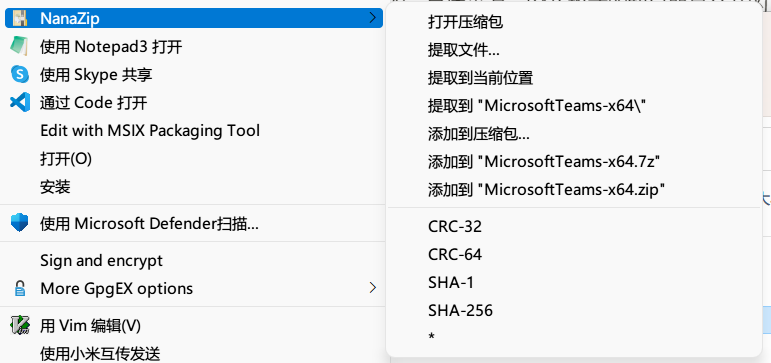
\includegraphics[width=9cm]{assets/Nanazip_Right_Click.png}
  \caption{NanaZip的右键菜单}
  \label{Nanazip_Right_Click}
\end{figure}

这些选项能帮助你解压压缩包、制作新的压缩包。例如上图中【提取到 “MicrosoftTeams-x64\textbackslash ”】就能把这个压缩包解压,再把其中的所有内容放在一个名叫「\verb|MicrosoftTeams-x64|」的文件夹下;
而上图中【添加到压缩包…】就可以将选中的文件压缩,具体用什么格式则会在后续的窗口中设定。

如果你直接双击打开一个压缩包,一般来说就可以直接查看其中的内容,而不解包这个压缩包:

\begin{figure}[htb!]
  \centering
  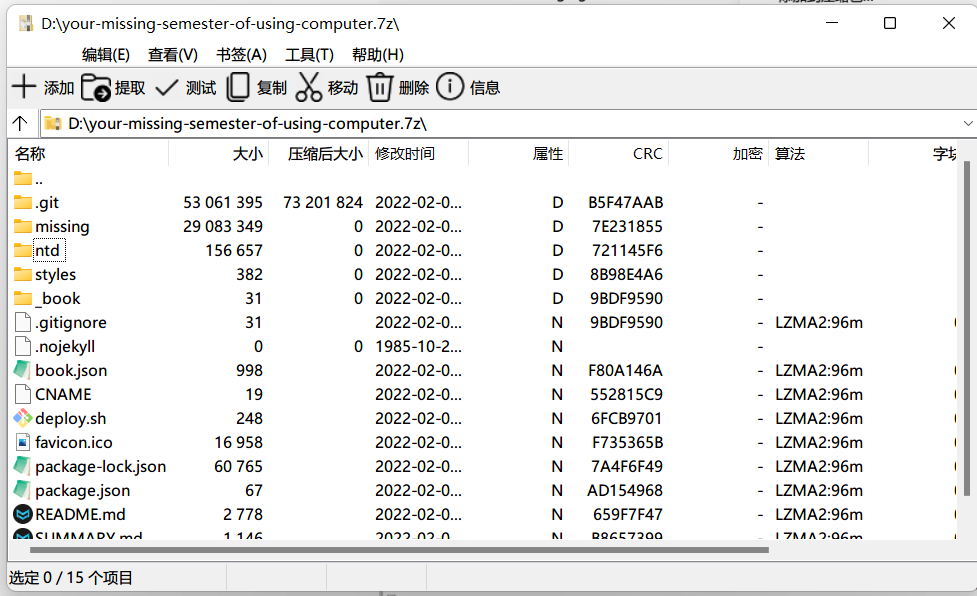
\includegraphics[width=8cm]{assets/Nanazip_View.png}
  \caption{打开的压缩文件}
  \label{Nanazip_View}
\end{figure}

如果你双击这份列表中的某一个文件,那么压缩工具一般会将\regcolor{这一个文件}(而不是整个压缩包)解压到一个\regcolor{临时位置},并将其打开。
这一切都是临时的,这个临时解压出来的文件会在你关闭它之后被销毁——因此,这种双击压缩包内某文件来打开它的方式\regcolor{只适用于临时预览压缩包中某一个文件的内容}。
所以,在运行以压缩包形式提供的应用程序时,请\regcolor{一定完全解压到某个干净的地方后再运行}!

通过「拖拽」的方式,则可以安全地将压缩包中的单独一个或几个文件解压到你想要的安全位置。
例如,如果你选中上图中的\verb|book.json|、\verb|favicon.ico|和\verb|package.json|三个文件,然后把它们拖拽到桌面,这三个文件就会被解压出来并放在桌面上。

\begin{note}
  压缩包是具有一定可编辑性的——这意味着,借助压缩工具,你可以往一个现有的压缩包中继续添加新的文件,也可以删除一个现有压缩包中的某个文件。
  具体的操作依压缩工具不同而有所差异,因而这里不再深入介绍。
\end{note}

下面我们介绍一些常见的压缩软件。

\subsection{7-Zip / NanaZip}

7-Zip 是 7z 格式的那帮作者亲自操刀做出来的压缩工具,它是一款自由软件。
除了 7z 格式之外,它还支持打开几乎所有格式(包含 RAR)的压缩包,并能制作 ZIP、TAR、GZ 等各种(不含 RAR)格式的压缩包。

7-Zip 软件比较小巧简洁,功能比较完善。其比较影响体验的缺点是外观——7-Zip 软件的默认界面风格相当的「复古」,如下图所示。

\begin{figure}[htb!]
  \centering
  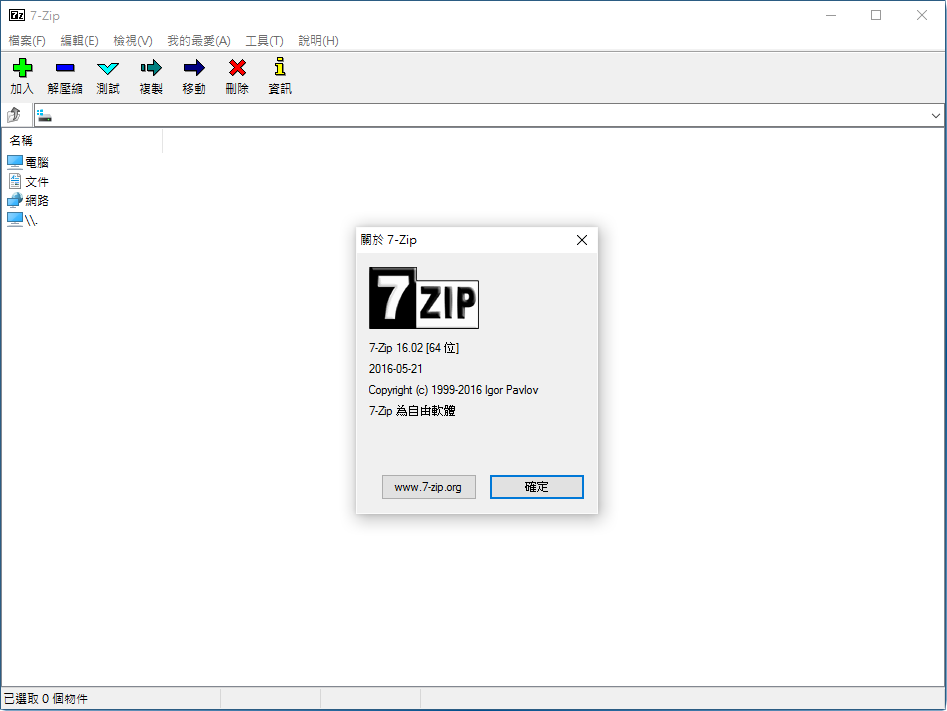
\includegraphics[width=8cm]{assets/7-Zip.png}
  \caption{7-Zip}
  \label{7-Zip}
\end{figure}

7-Zip 的官方下载地址是 \url{https://www.7-zip.org/}。
如果访问这个链接有困难,可以选择 \url{https://sparanoid.com/lab/7z/}。

由于 7-Zip 的界面复古,且不支持 Windows 11 的新式右键菜单(参见\nameref{windows-11-optimization}),一些有志之士在 7-Zip 的基础上开发了 NanaZip。
现阶段(2022 年初),NanaZip 可以看成是换了好看主题并且支持 Windows 11 新式右键菜单的 7-Zip。
下面是 NanaZip 的界面。

\begin{figure}[htb!]
  \centering
  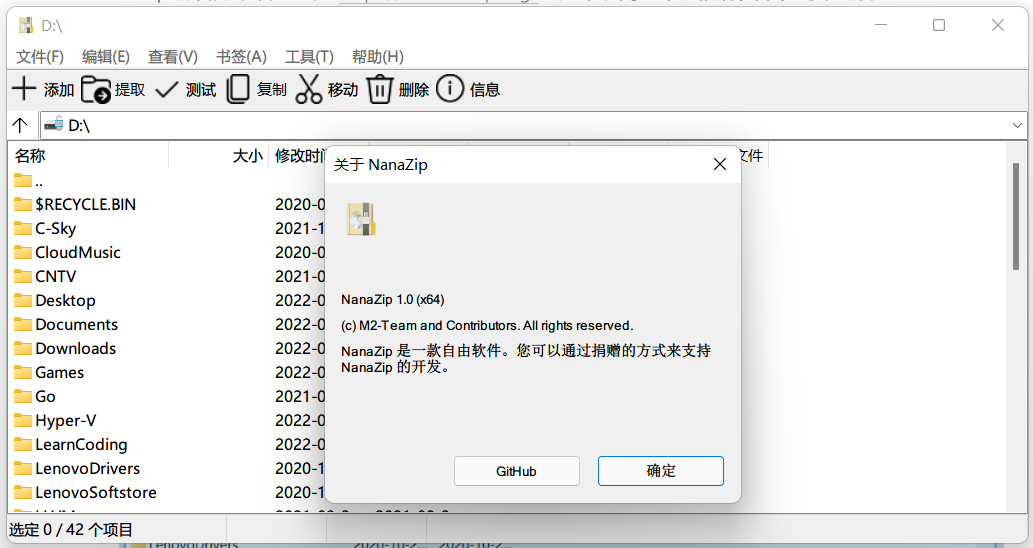
\includegraphics[width=9cm]{assets/NanaZip.png}
  \caption{NanaZip}
  \label{NanaZip}
\end{figure}

NanaZip 可以在 Microsoft Store 搜索「NanaZip」直接安装。
或者,你也可以在 \url{https://github.com/M2Team/NanaZip/releases} 手动下载安装它。

\subsection{Bandizip}

Bandizip 是由 Bandisoft 开发的一款压缩软件,有免费的标准版与付费的专业版、企业版。
免费版可以在 \url{https://www.bandisoft.com/bandizip/} 下载到。
它也支持读取几乎所有格式的压缩包,也能制作包括但不限于常见的 ZIP、7Z 格式,以及不常见的 TAR 等格式的压缩包。
当然,和 7-Zip 一样,Bandizip 无法制作 RAR 压缩包。

Bandizip的主界面大致如下图所示。
可以看见,它的界面较为简洁、现代,但美中不足的便是右下角的广告。
这广告需要我们购买专业版或企业版才能去除,不过实际使用上却几乎没有干扰,因为广告仅在没有打开任何文件时出现,而实际使用时我们基本上不会来到这里。

\begin{figure}[htb!]
  \centering
  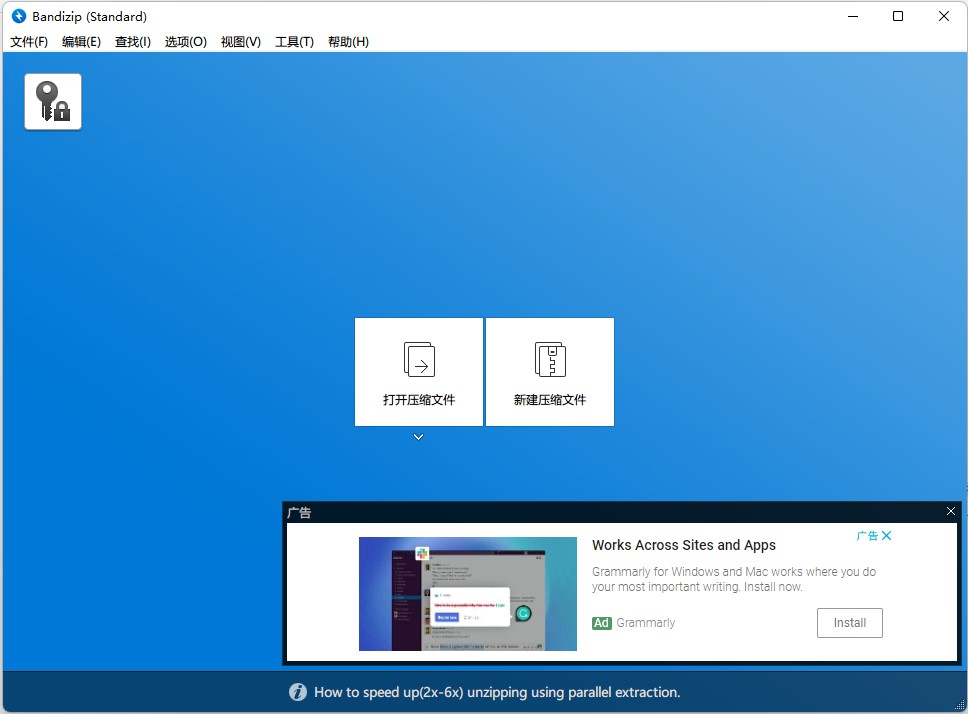
\includegraphics[width=9cm]{assets/Bandizip.jpg}
  \caption{Bandizip}
  \label{Bandizip}
\end{figure}

当你使用 Bandizip 打开一个压缩文件时,软件界面大致如下图。
这里是没有广告的。
你可以在此对压缩文件进行各种操作。

\begin{figure}[htb!]
  \centering
  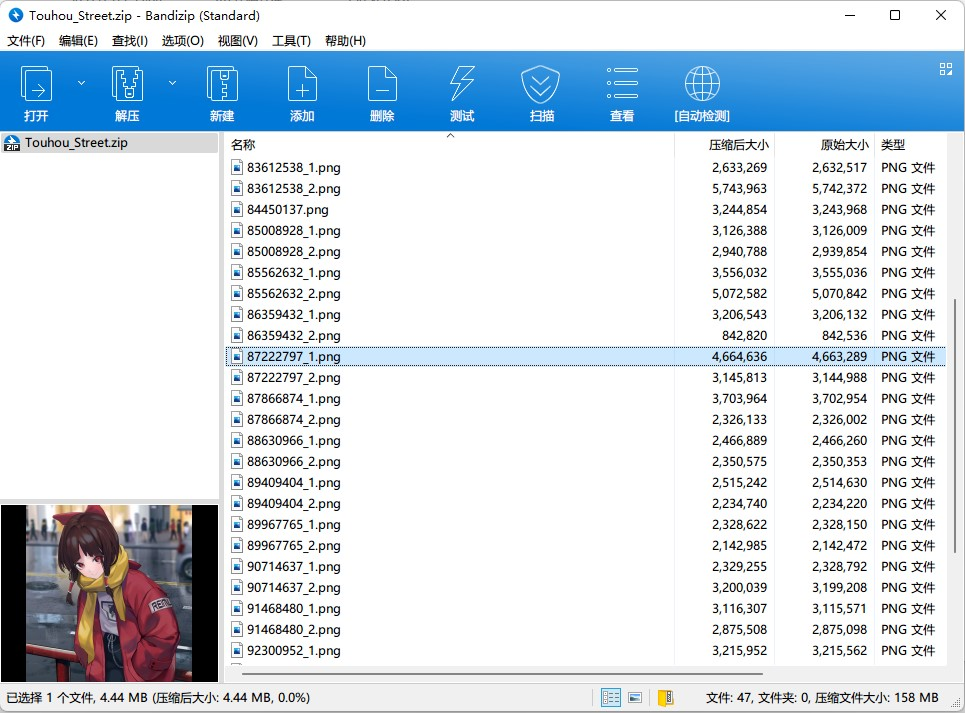
\includegraphics[width=9.5cm]{assets/Bandizip_View.jpg}
  \caption{用Bandizip打开文件}
  \label{Bandizip_View}
\end{figure}

Bandizip 值得一提的两个功能,一是「压缩文件预览」,二是「自动解压」。

「压缩文件预览」是说,当你右击一个压缩文件时,若这个文件没怎么加密\footnote{压缩文件的加密大体上有两种情况:一种是比较完全,这种压缩文件如果不输入密码,就连里边压缩的文件的名字也无法读取;另一种则相对宽松,在不输入密码的时候,也可以打开这个压缩包去查看里面有哪些文件(尽管不能把它们解压出来)。},你的右键菜单便会显示出这个压缩包内部的部分文件;
若是连文件名都加密了,那当然什么都看不见啦。
可惜这个功能只支持旧式菜单,不支持 Windows 11 的新式菜单。

\begin{figure}[htb!]
  \centering
  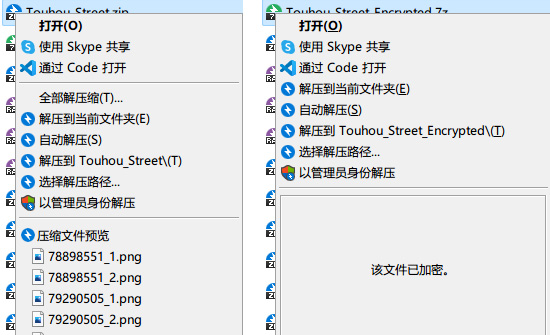
\includegraphics[width=8cm]{assets/Compressed_Preview.jpg}
  \caption{「压缩文件预览」右键菜单}
  \label{Compressed_Preview}
\end{figure}

「自动解压」则是一种「傻瓜式解压操作」。
还记得\nameref{files-and-file-management}中我们介绍的「解压到当前文件夹」和「解压到 xxxxxx\textbackslash 」的区别吗?
「自动解压」能够自动在这两种模式中选择更合适的那个——当你的压缩文件根目录仅有一个文件或文件夹时,Bandizip 便选择「解压到当前文件夹」;
若有多个文件 / 文件夹, Bandizip 则会选择「解压到 xxxxxx\textbackslash」。

举个简单的例子:上图中的压缩包内部就有许多图片,假设这个压缩包所在的路径是「\verb|D:\Touhou_Street.zip|」,点击【自动解压】,那么图片就会被提取到「\verb|D:\Touhou_Street\|」下;
若这压缩包里面就一张图,则会被提取到「\verb|D:\|」下。

「自动解压」既支持旧式右键菜单也支持 Windows 11 的新式右键菜单,若使用 Bandizip,我们建议始终使用「自动解压」来解压文件,除非你有特殊目的。

\begin{figure}[htb!]
  \centering
  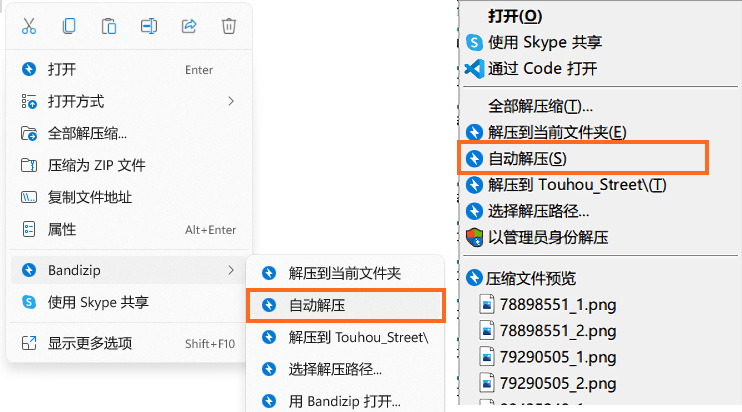
\includegraphics[width=9cm]{assets/Auto_Decompress.jpg}
  \caption{「自动解压」右键菜单}
  \label{Auto_Decompress}
\end{figure}

\subsection{WinRAR}

WinRAR 是 RAR 格式的作者设计的软件。
顾名思义,WinRAR 最大的特点就是「RAR」——它(可能)是 Windows 平台上唯一一款能够支持制作 RAR 格式压缩包的压缩软件。
除了 RAR 格式外,它也支持 ZIP、7z、TAR 等各种其他压缩格式的压缩和解压。
WinRAR 的软件界面如下图所示。

\begin{figure}[htb!]
  \centering
  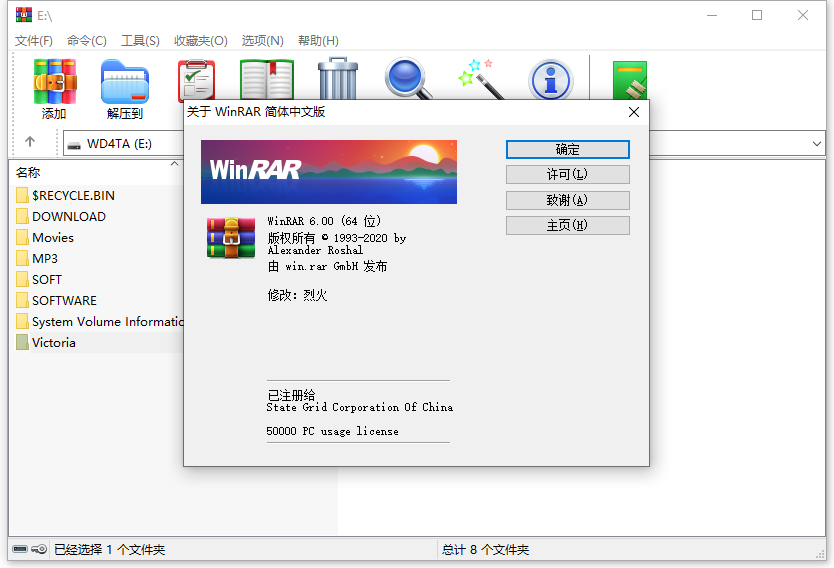
\includegraphics[width=8cm]{assets/WinRAR.png}
  \caption{WinRAR}
  \label{WinRAR}
\end{figure}

WinRAR 是收费的商业软件——换言之,这款软件需要购买才能合法使用。
WinRAR 在中国也提供了一个「个人免费版本」,这个版本包含恶性弹窗广告——与 Bandizip 那种不同,WinRAR 的广告在打开压缩文件的时候也会弹出。
如果你能接受那样的弹窗广告,那么 WinRAR 也许是一个不错的选择。

WinRAR 的国际官网是 \url{https://www.rarlab.com/},但如果要下载「个人免费版」,请访问 WinRAR 国内代理官网 \url{http://www.winrar.com.cn/index.htm}。

\subsection{国产压缩软件}

最后我们再来介绍一下压缩软件中的「深水区」——国产压缩软件们。
和\nameref{browsers-and-how-to-choose}一样,国产压缩软件也良莠不齐,其中不乏佳作也不少流氓软件。
由于除了 RAR 之外的几乎所有压缩格式都是公开的,因此几乎所有的国产压缩软件都和前文介绍的 7-Zip 或 Bandizip 一样,支持绝大多数格式压缩文件的解压,但不支持 RAR 格式压缩文件的制作。
例如,下面是「360 压缩」的客服人员对「『360 压缩』能否压缩 RAR 格式」这一问题的答复:

\begin{figure}[htb!]
  \centering
  
\includegraphics[width=12cm]{assets/360_Zip.png}
  \caption{「360 压缩」能否压缩 RAR 格式?}
  \label{360_Zip}
\end{figure}

与「360 压缩」这种勉强还能说「好用」的国产压缩软件相比,「2345 好压」「快压」等则表现出了许多流氓软件的特征——静默捆绑安装、大量的广告推送,以及难以卸载和清除。
总而言之,和前文介绍浏览器时我们的态度一样,对于国产压缩软件,我们建议各取所需,审慎行事。

\practice

\begin{enumerate}
  \item 简要用自己的话复述「压缩」这个过程。
  \item 自己制作几个压缩文件,然后分别用「解压到当前文件夹」「解压到 xxxxxx\textbackslash 」来解压它们,体会这两种解压方式的区别。思考 Bandizip 的「自动解压」到底有多「自动」。
  \item 你正在使用什么压缩软件?它的使用体验(界面美观度、操作难易度、是否有广告……)如何?
\end{enumerate}